%%%%%%%%%%%%%%%%%%%%%%%%%%%%%%%%%%%%%%%%%
% Beamer Presentation
% LaTeX Template
% Version 1.0 (10/11/12)
%
% This template has been downloaded from:
% http://www.LaTeXTemplates.com
%
% License:
% CC BY-NC-SA 3.0 (http://creativecommons.org/licenses/by-nc-sa/3.0/)
%
%%%%%%%%%%%%%%%%%%%%%%%%%%%%%%%%%%%%%%%%%

%----------------------------------------------------------------------------------------
%	PACKAGES AND THEMES
%----------------------------------------------------------------------------------------

\documentclass{beamer}

\mode<presentation> {

% The Beamer class comes with a number of default slide themes
% which change the colors and layouts of slides. Below this is a list
% of all the themes, uncomment each in turn to see what they look like.

%\usetheme{default}
%\usetheme{AnnArbor}
%\usetheme{Antibes}
%\usetheme{Bergen}
%\usetheme{Berkeley}
%\usetheme{Berlin}
%\usetheme{Boadilla}
%\usetheme{CambridgeUS}
%\usetheme{Copenhagen}
%\usetheme{Darmstadt}
%\usetheme{Dresden}
%\usetheme{Frankfurt}
%\usetheme{Goettingen}
%\usetheme{Hannover}
%\usetheme{Ilmenau}
%\usetheme{JuanLesPins}
%\usetheme{Luebeck}
\usetheme{Madrid}
%\usetheme{Malmoe}
%\usetheme{Marburg}
%\usetheme{Montpellier}
%\usetheme{PaloAlto}
%\usetheme{Pittsburgh}
%\usetheme{Rochester}
%\usetheme{Singapore}
%\usetheme{Szeged}
%\usetheme{Warsaw}

% As well as themes, the Beamer class has a number of color themes
% for any slide theme. Uncomment each of these in turn to see how it
% changes the colors of your current slide theme.

%\usecolortheme{albatross}
%\usecolortheme{beaver}
%\usecolortheme{beetle}
%\usecolortheme{crane}
%\usecolortheme{dolphin}
%\usecolortheme{dove}
%\usecolortheme{fly}
%\usecolortheme{lily}
%\usecolortheme{orchid}
%\usecolortheme{rose}
%\usecolortheme{seagull}
%\usecolortheme{seahorse}
%\usecolortheme{whale}
%\usecolortheme{wolverine}

%\setbeamertemplate{footline} % To remove the footer line in all slides uncomment this line
%\setbeamertemplate{footline}[page number] % To replace the footer line in all slides with a simple slide count uncomment this line

%\setbeamertemplate{navigation symbols}{} % To remove the navigation symbols from the bottom of all slides uncomment this line
}
%\usepackage{listings}
\usepackage{xcolor}
\usepackage{graphicx} % Allows including images
\usepackage{booktabs} % Allows the use of \toprule, \midrule and \bottomrule in tables
\usepackage{tcolorbox}
%----------------------------------------------------------------------------------------
%	TITLE PAGE
%----------------------------------------------------------------------------------------

\title[NP Pruning]{NP Pruning}

\author{Chris Pollard, Paul Mullen, \underline{Alexander Morton}} % Your name
\institute[Glasgow] % Your institution as it will appear on the bottom of every slide, may be shorthand to save space
{
University of Glasgow \\ % Your institution for the title page
\medskip
\textit{a.morton.2@research.com} % Your email address
}
\date{\today} % Date, can be changed to a custom date

\begin{document}

\begin{frame}
\frametitle{0 Lepton Merged}
\begin{columns}[t]
\column{0.5\textwidth}
\centering
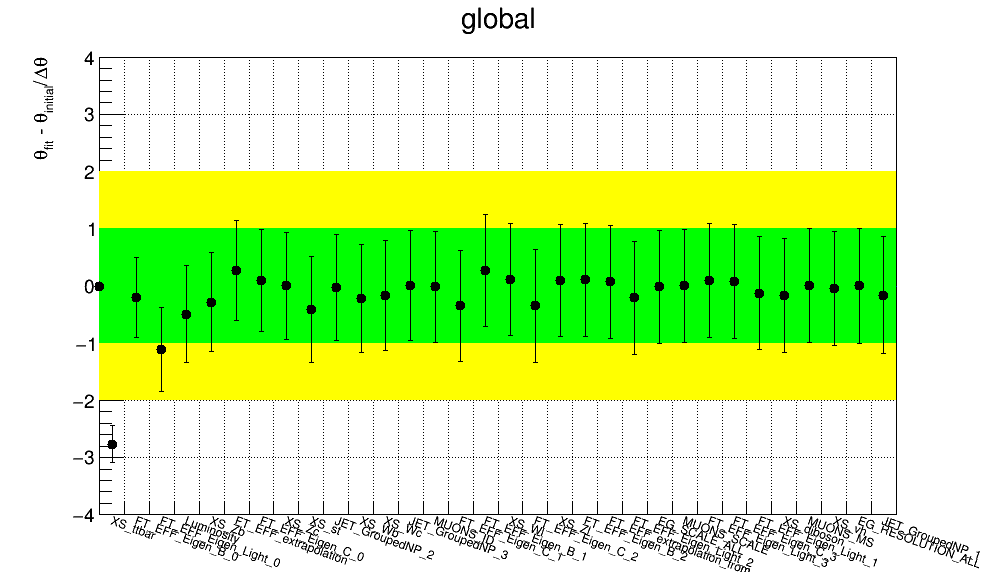
\includegraphics[width=0.8\linewidth]{pics/pull_0lep_merge_order_constraint.png}\\
\tiny{ Ordered by NP constraint }\\
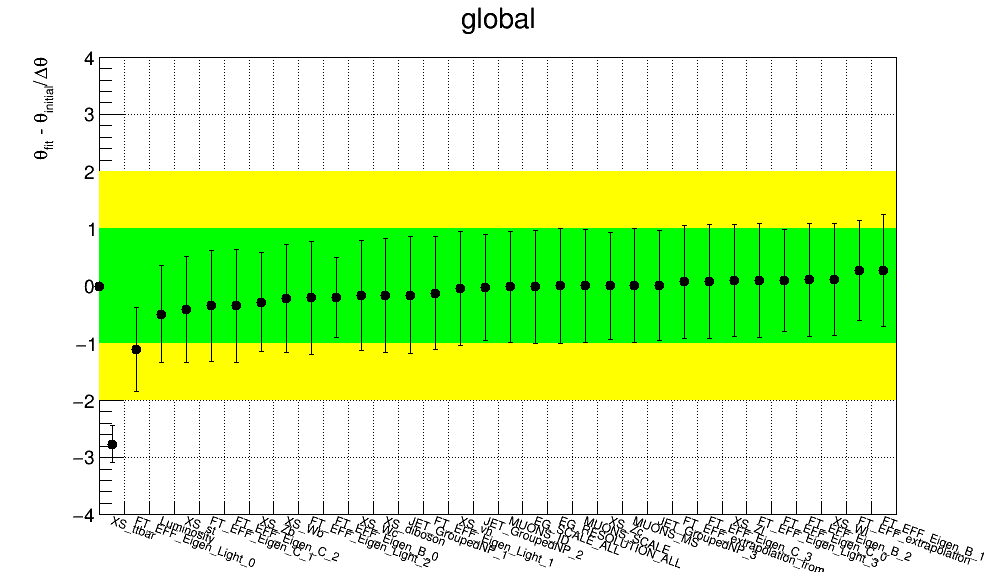
\includegraphics[width=0.8\linewidth]{pics/pull_0lep_merge_order_pull.png}\\
\tiny{ Order by pulls  }\\
\column{0.5\textwidth}
\centering
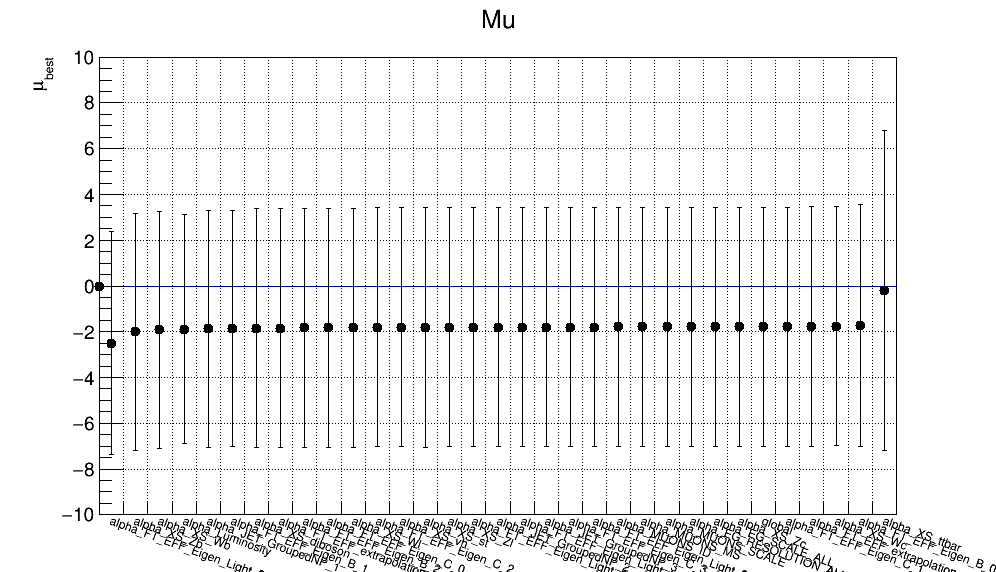
\includegraphics[width=0.8\linewidth]{pics/mu_0lep_merge_order_pull.png}\\
\tiny{ Order by pull }\\
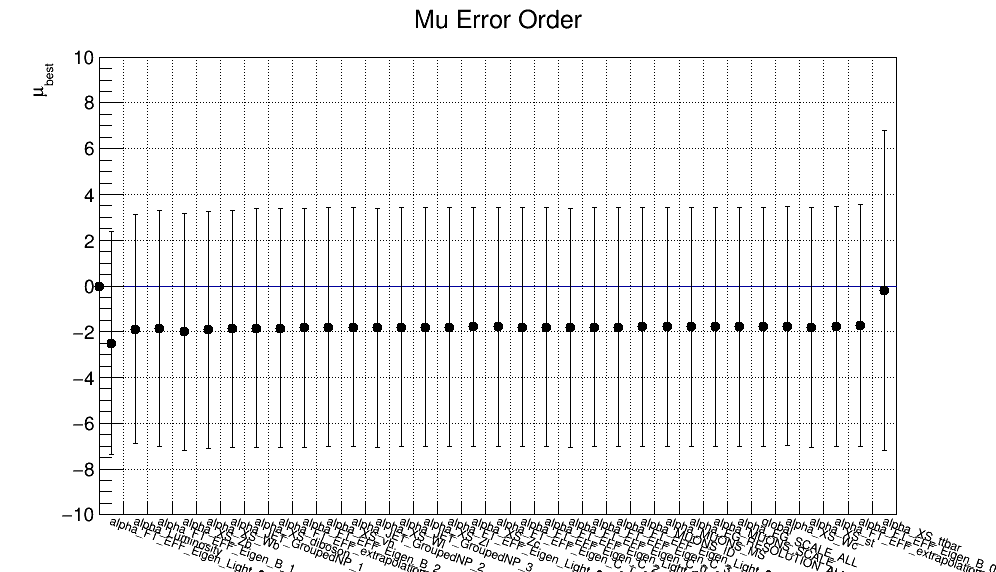
\includegraphics[width=0.8\linewidth]{pics/mu_0lep_merge_order_constraint.png}\\ 
\tiny{ Order by constraint }\\
\end{columns}
\end{frame}

\begin{frame}
\frametitle{1 Lepton Merged}
\begin{columns}[t]
\column{0.5\textwidth}
\centering
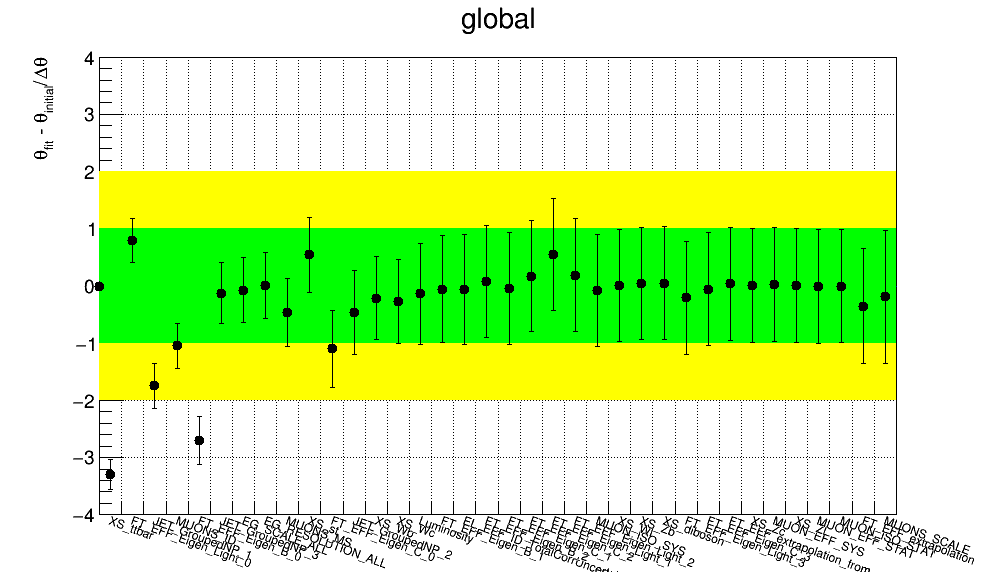
\includegraphics[width=0.8\linewidth]{pics/pull_1lep_merge_order_constraint.png}\\
\tiny{ Ordered by NP constraint }\\
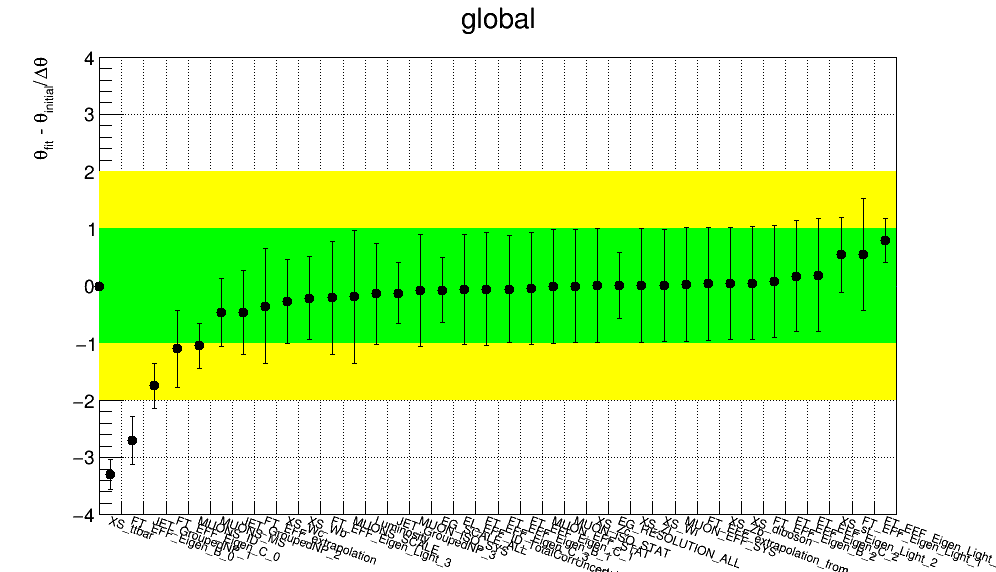
\includegraphics[width=0.8\linewidth]{pics/pull_1lep_merge_order_pull.png}\\
\tiny{ Order by pulls  }\\
\column{0.5\textwidth}
\centering
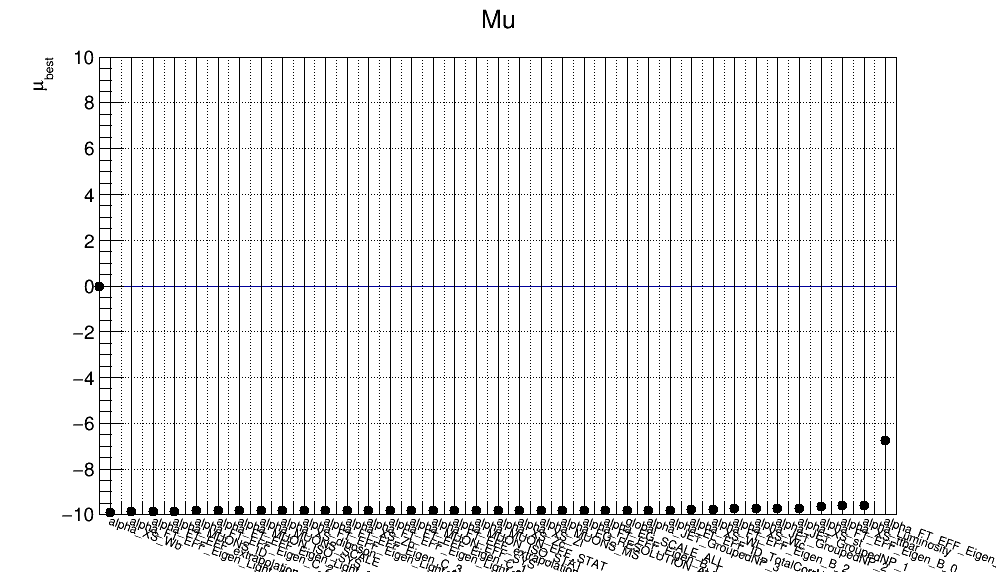
\includegraphics[width=0.8\linewidth]{pics/mu_1lep_merge_order_pull.png}\\
\tiny{ Order by pull }\\
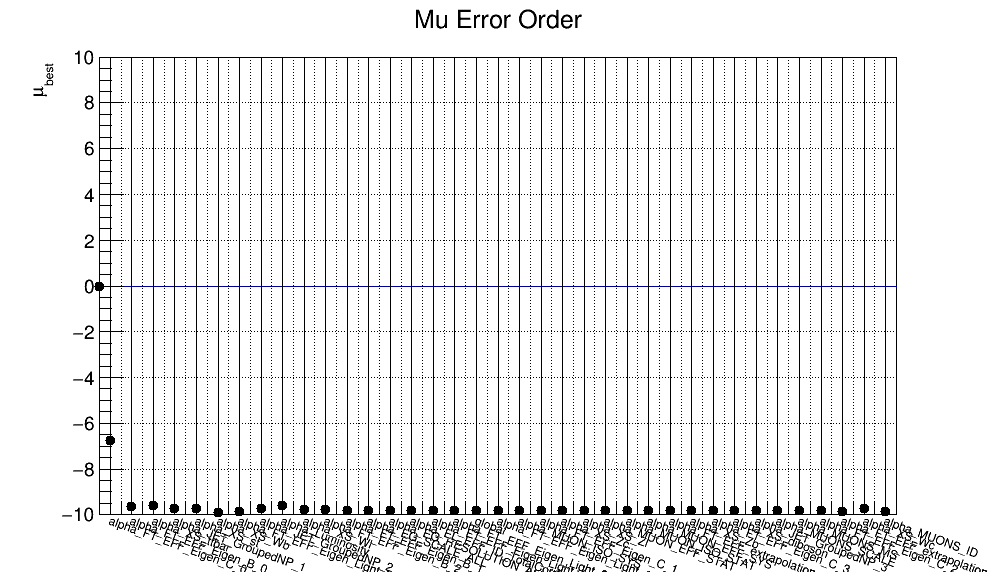
\includegraphics[width=0.8\linewidth]{pics/mu_1lep_merge_order_constraint.png}\\ 
\tiny{ Order by constraint }\\
\end{columns}
\end{frame}

\begin{frame}
\frametitle{2 Lepton Merged}
\begin{columns}[t]
\column{0.5\textwidth}
\centering
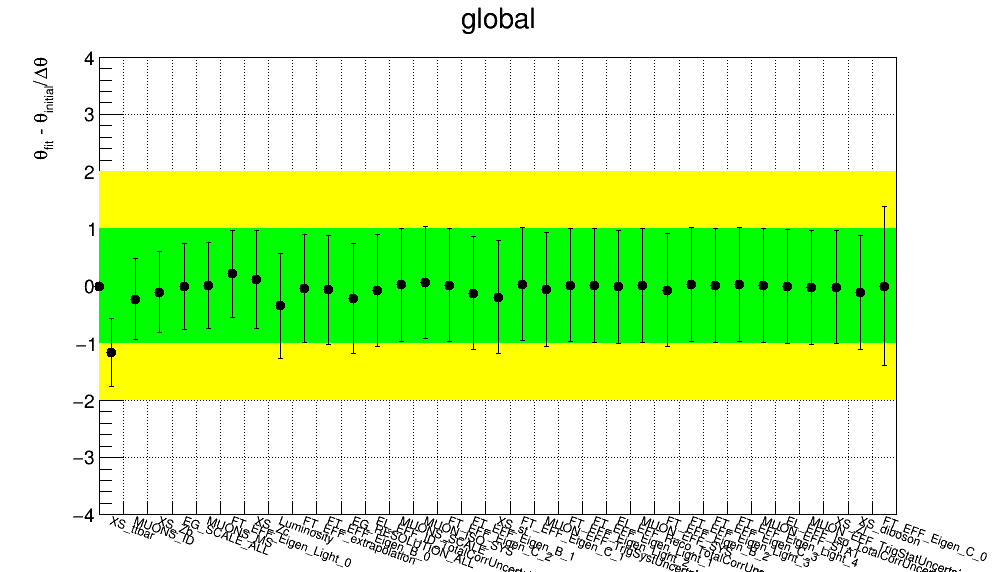
\includegraphics[width=0.8\linewidth]{pics/pull_2lep_merge_order_constraint.png}\\
\tiny{ Ordered by NP constraint }\\
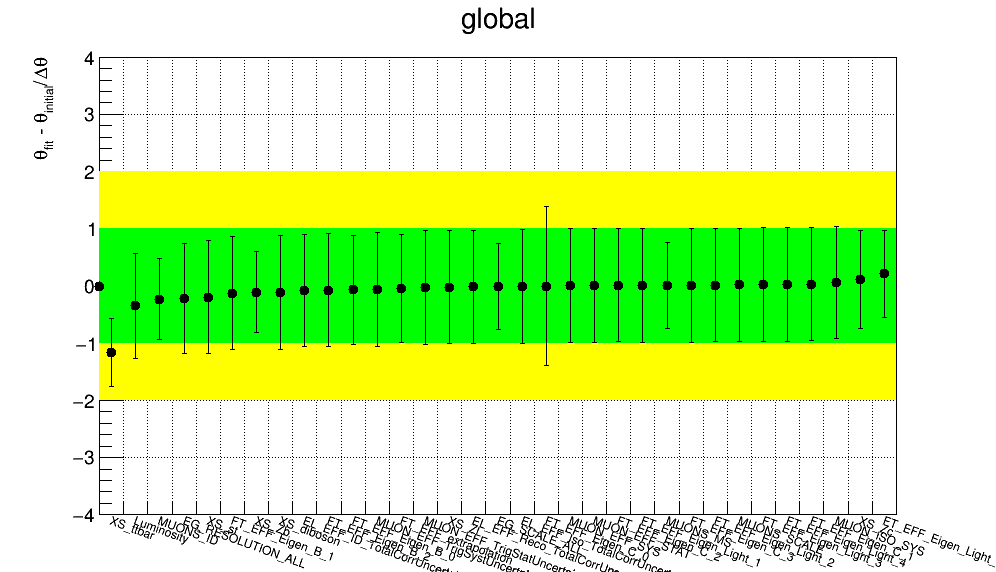
\includegraphics[width=0.8\linewidth]{pics/pull_2lep_merge_order_pull.png}\\
\tiny{ Order by pulls  }\\
\column{0.5\textwidth}
\centering
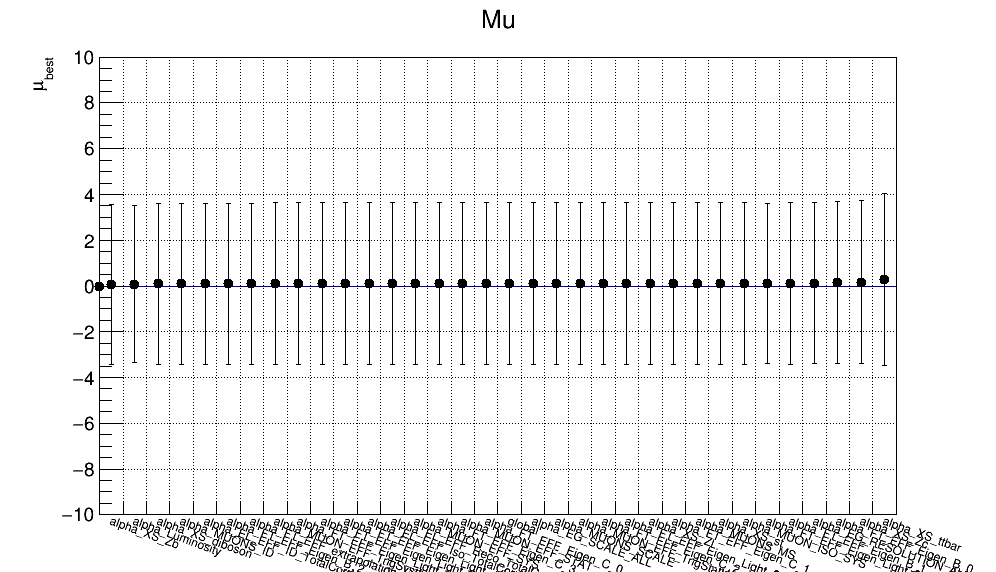
\includegraphics[width=0.8\linewidth]{pics/mu_2lep_merge_order_pull.png}\\
\tiny{ Order by pull }\\
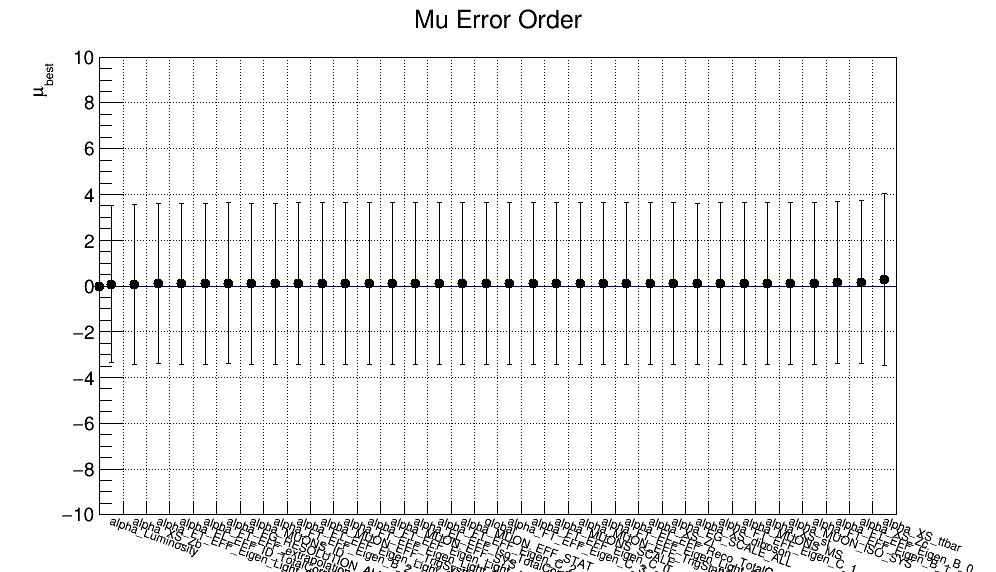
\includegraphics[width=0.8\linewidth]{pics/mu_2lep_merge_order_constraint.png}\\ 
\tiny{ Order by constraint }\\
\end{columns}
\end{frame}

\begin{frame}
\frametitle{Chi2}
\begin{columns}[t]
\column{0.5\textwidth}
\centering
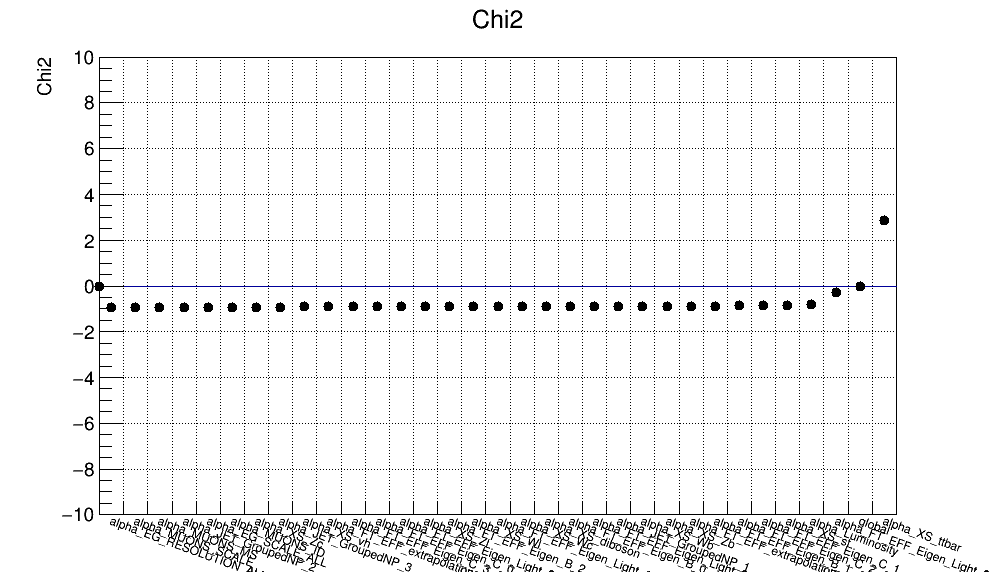
\includegraphics[width=0.8\linewidth]{pics/chi_0lep_merge.png}\\
\tiny{ 0 lepton }\\
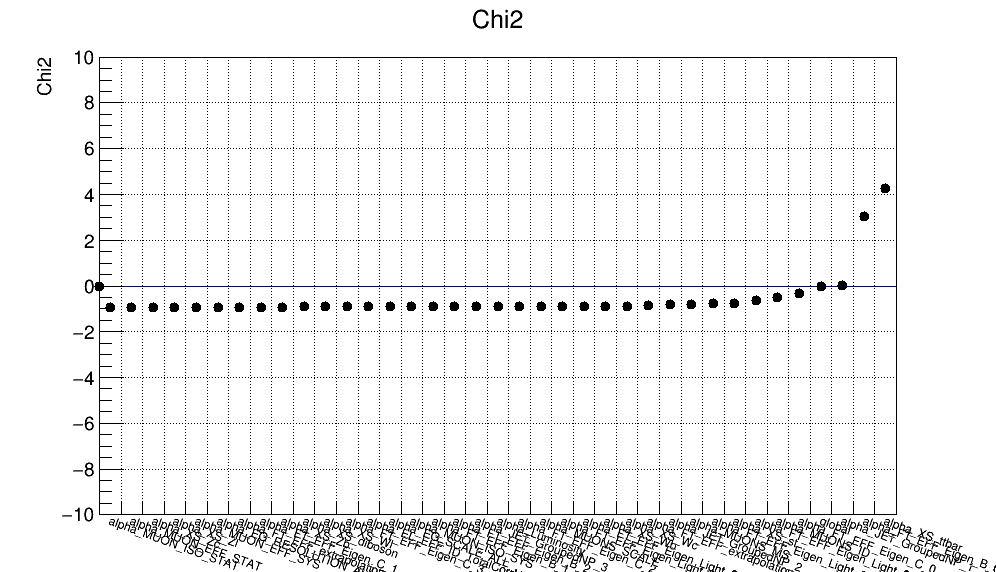
\includegraphics[width=0.8\linewidth]{pics/chi_1lep_merge.png}\\
\tiny{ 1 lepton  }\\
\column{0.5\textwidth}
\centering
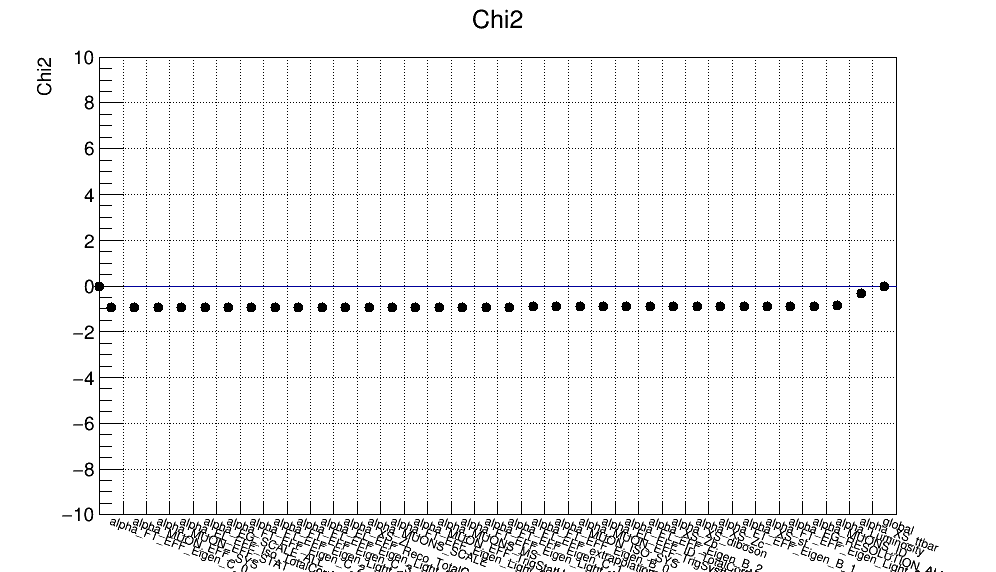
\includegraphics[width=0.8\linewidth]{pics/chi_2lep_merge.png}\\
\tiny{ 2 lepton }\\

\end{columns}
\end{frame}

\end{document}
\begin{frame}
\frametitle{Chi2/Ndof with different NP}
\begin{columns}[t]
\column{0.5\textwidth}
\centering
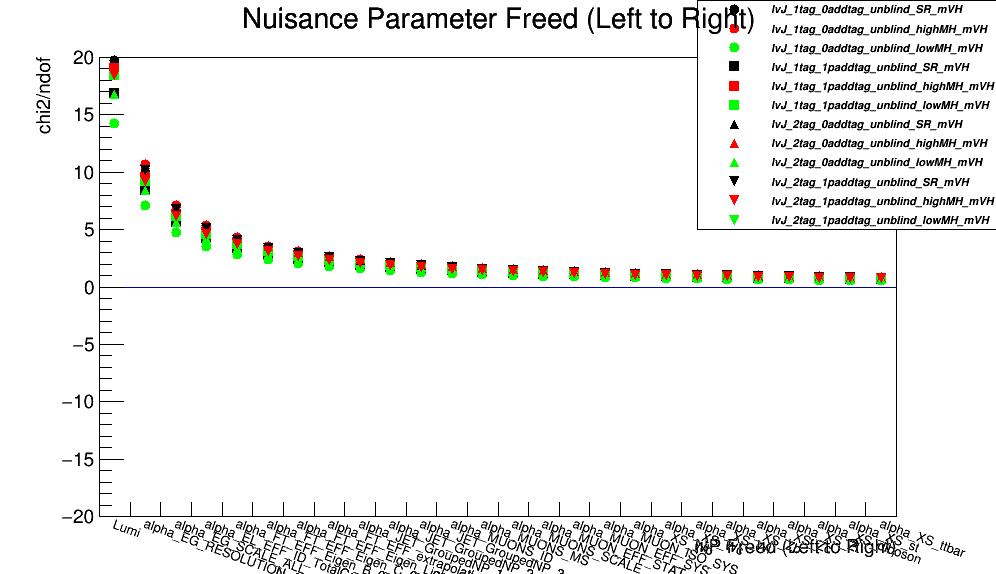
\includegraphics[width=0.8\linewidth]{pics/nui_largeScale.png}\\
\tiny{ No failed fits, i.e all non negative }\\
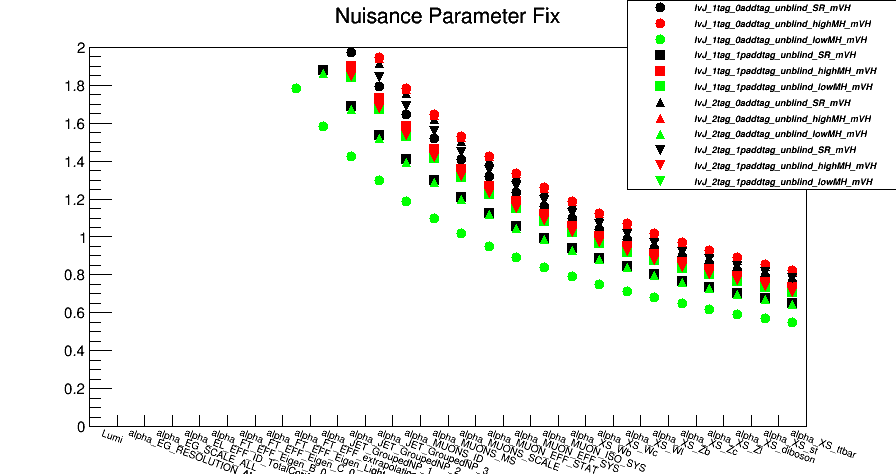
\includegraphics[width=0.8\linewidth]{pics/nui.png}\\
\tiny{ Closer to 1  }\\
\column{0.5\textwidth}
\centering
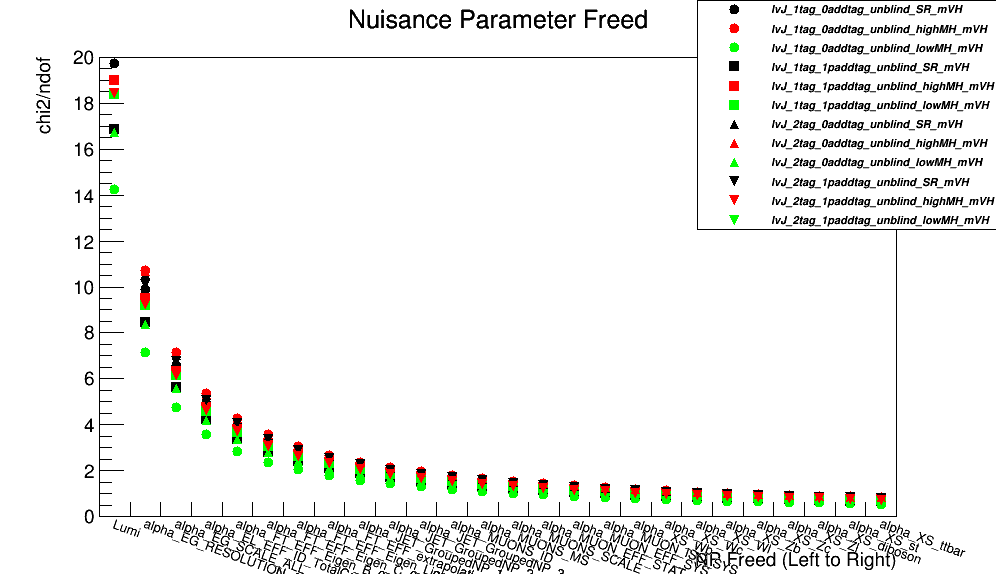
\includegraphics[width=0.8\linewidth]{pics/nui_largeScaleNonNeg.png}\\
\tiny{ The full range. }\\
\includegraphics[width=0.8\linewidth]{pics/Sig_1000_2000_3000_Mass_log.png}\\ 
%\tiny{ Mass (Log) }\\
\end{columns}
\end{frame}

\begin{frame}
\frametitle{Chi2/Ndof and POI with different NP Fixed (Only 1 fixed each time)}
\begin{columns}[t]
\column{0.5\textwidth}
\centering
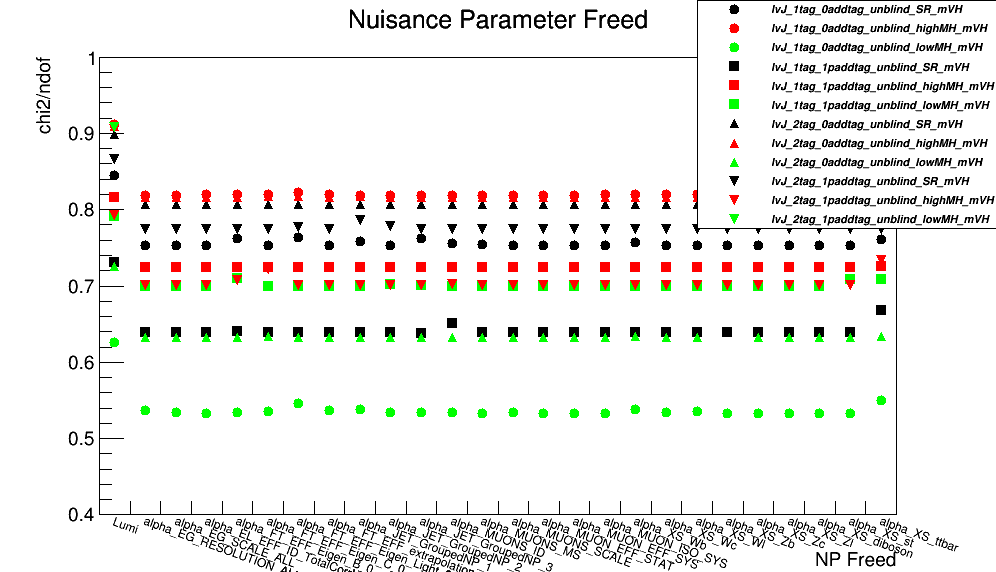
\includegraphics[width=0.8\linewidth]{pics/nui_OneNui2.png}\\
\tiny{ Single NP fixed . }\\
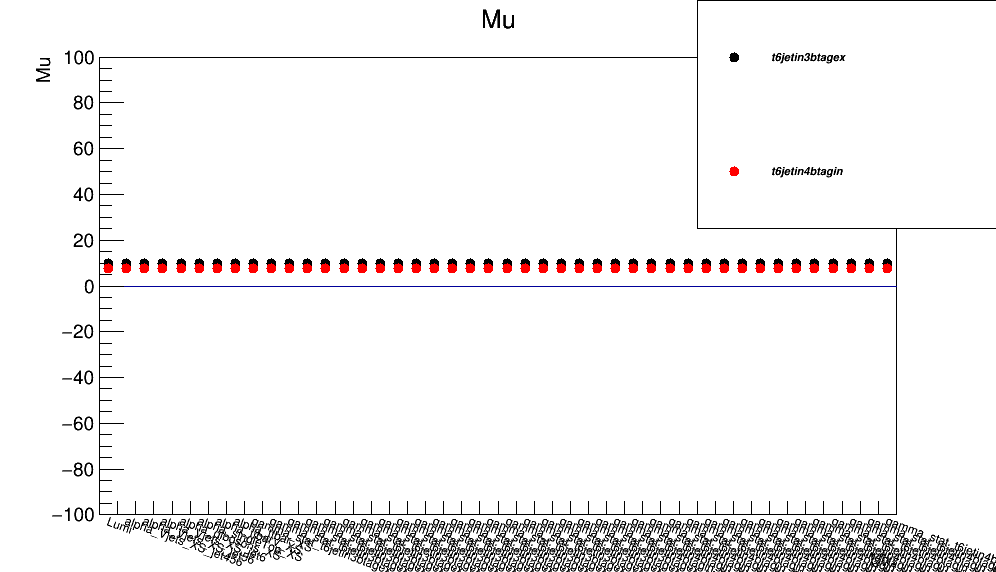
\includegraphics[width=0.8\linewidth]{pics/mu_test.png}\\
\tiny{ Example WS with nuissance check. Appears constant?  }\\
\column{0.5\textwidth}
\centering
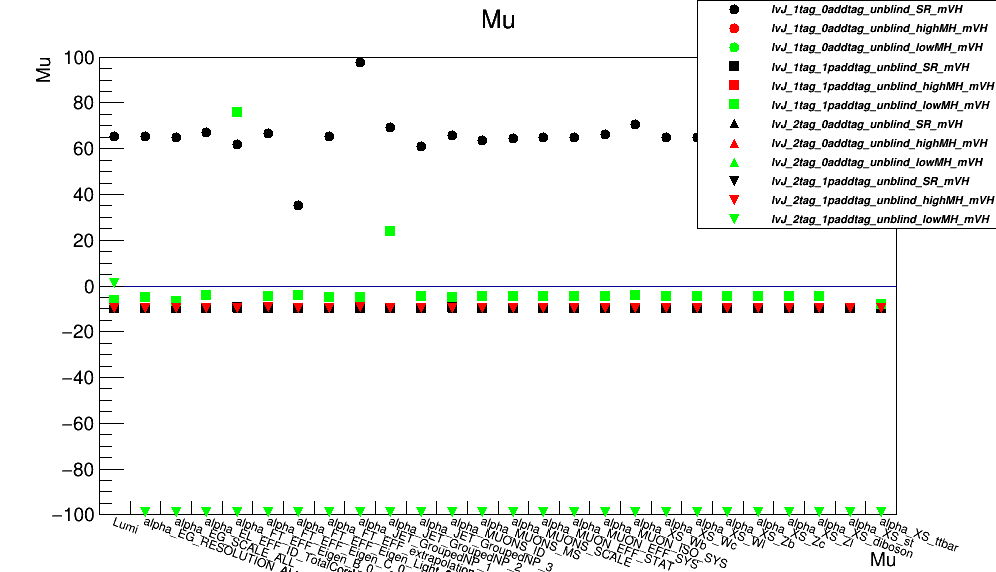
\includegraphics[width=0.8\linewidth]{pics/mu.png}\\
\tiny{ Mu for our workspace. }\\
%\includegraphics[width=0.8\linewidth]{pics/Sig_1000_2000_3000_Mass_log.png}\\ 
%\tiny{ Mass (Log) }\\
\end{columns}
\end{frame}

\begin{frame}
\frametitle{2 Lepton. 2TeV}
\begin{columns}[t]
\column{0.5\textwidth}
\centering
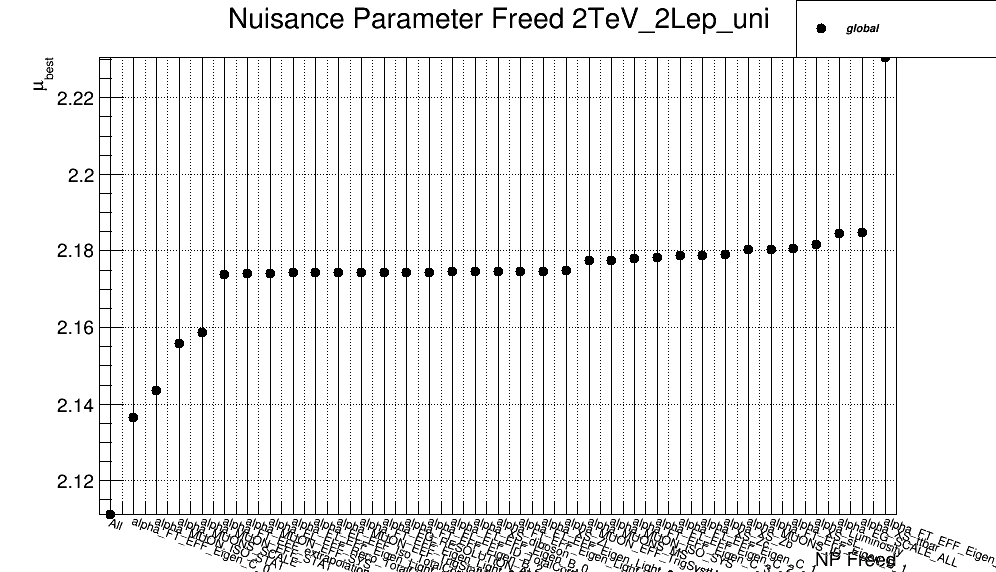
\includegraphics[width=0.8\linewidth]{pics/globalFitMu_2TeV_2Lep_uni.png}\\
\tiny{ Uniform 2 Lep. Mu }\\
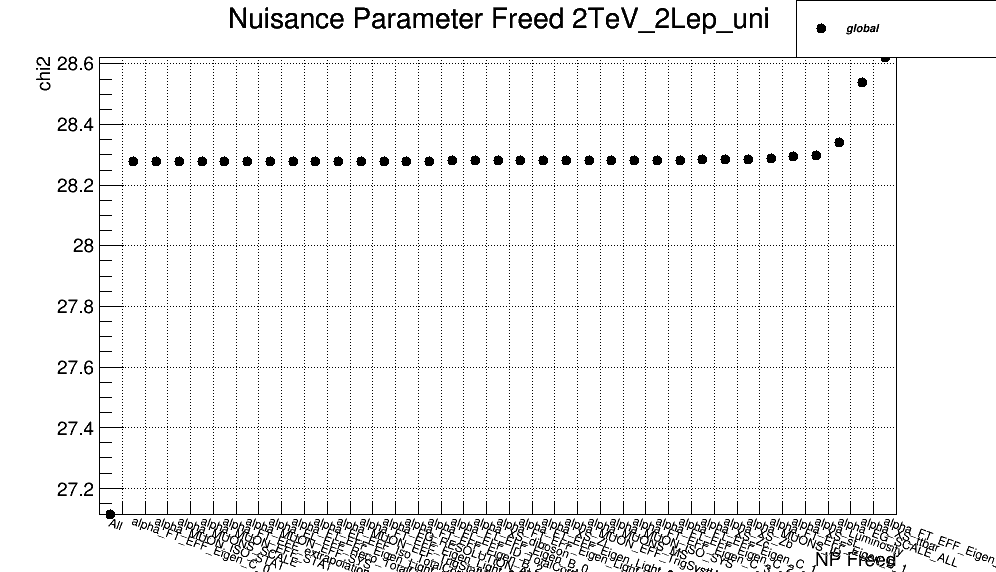
\includegraphics[width=0.8\linewidth]{pics/globalFitChi2_2TeV_2Lep_uni_.png}\\
\tiny{ Uniform 2 Lep chi2  }\\
\column{0.5\textwidth}
\centering
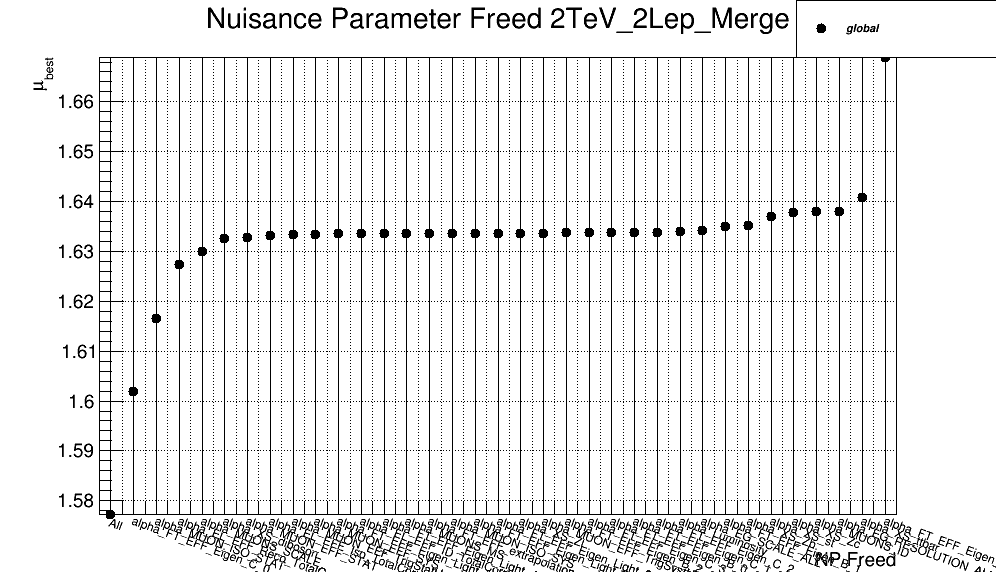
\includegraphics[width=0.8\linewidth]{pics/globalFitMu_2TeV_2Lep_Merge.png}\\
\tiny{ Merge 2 Lep. Mu }\\
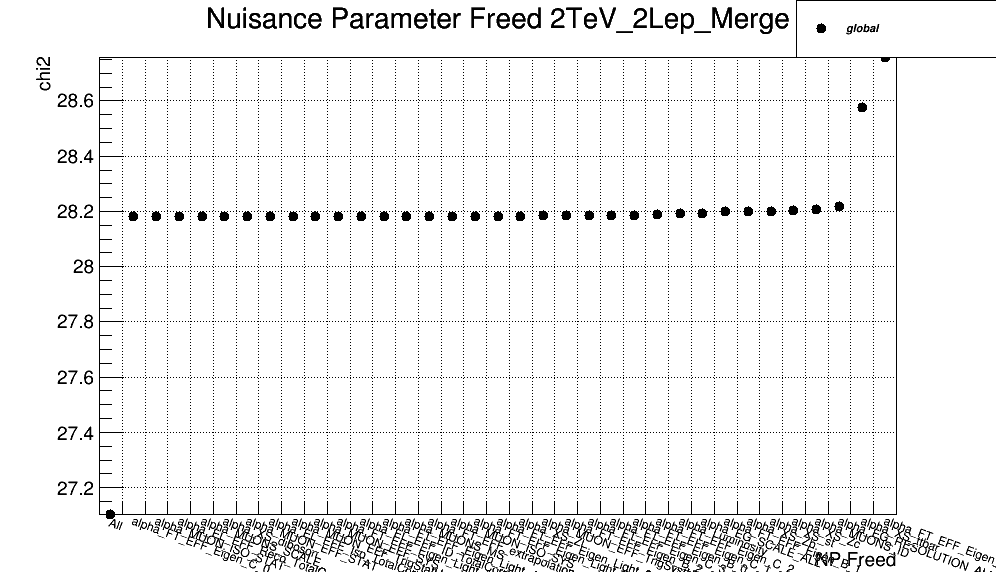
\includegraphics[width=0.8\linewidth]{pics/globalFitChi2_2TeV_2Lep_Merge_.png}\\ 
\tiny{ Merge 2 Lep. Chi2 }\\
\end{columns}
\end{frame}


\begin{frame}
\frametitle{0 Lepton. 2TeV}
\begin{columns}[t]
\column{0.5\textwidth}
\centering
%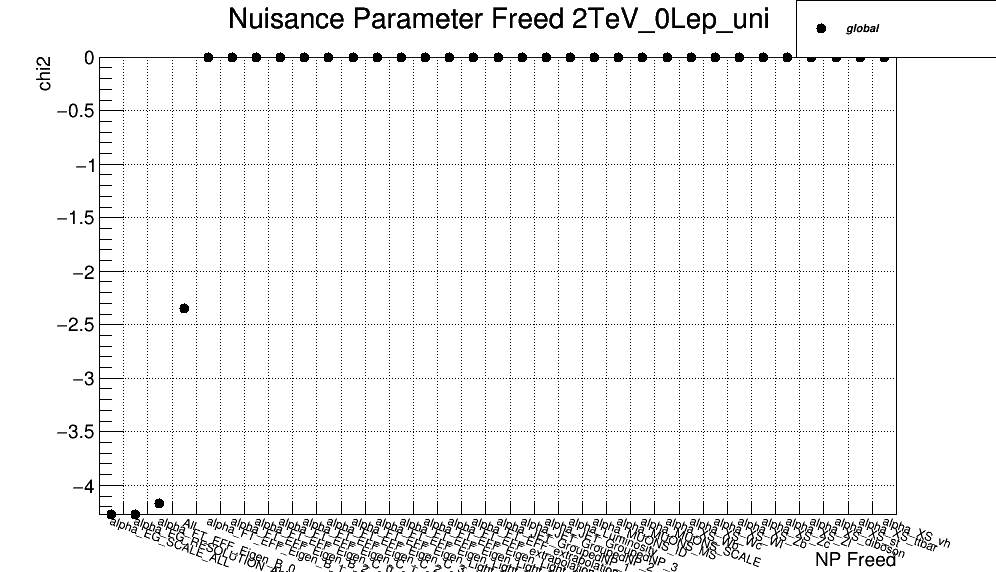
\includegraphics[width=0.8\linewidth]{pics/globalFitMu_2TeV_0Lep_uni.png}\\
\tiny{ Uniform Mu }\\
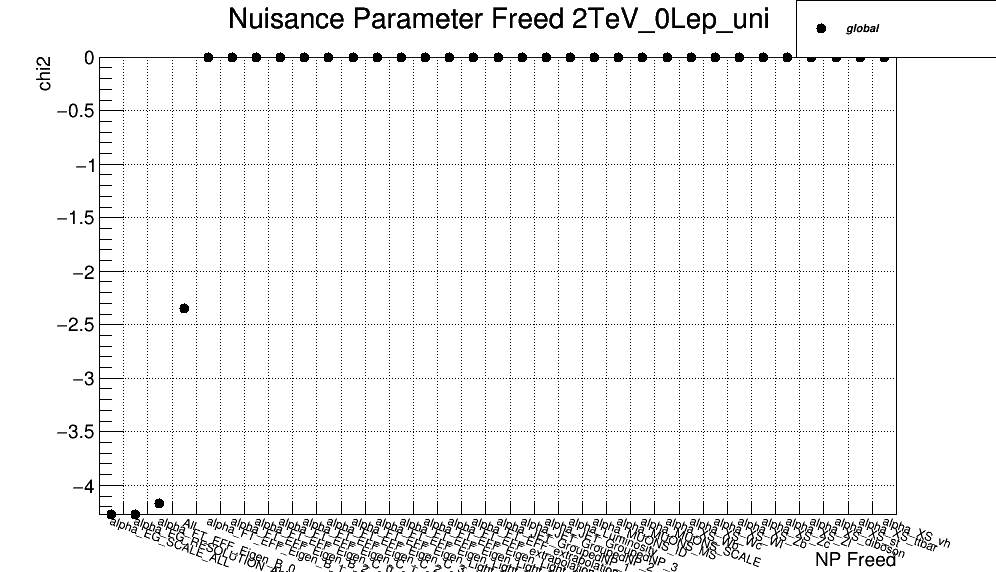
\includegraphics[width=0.8\linewidth]{pics/globalFitChi2_2TeV_0Lep_uni_.png}\\
\tiny{ Uniform. chi2  }\\
\column{0.5\textwidth}
\centering
%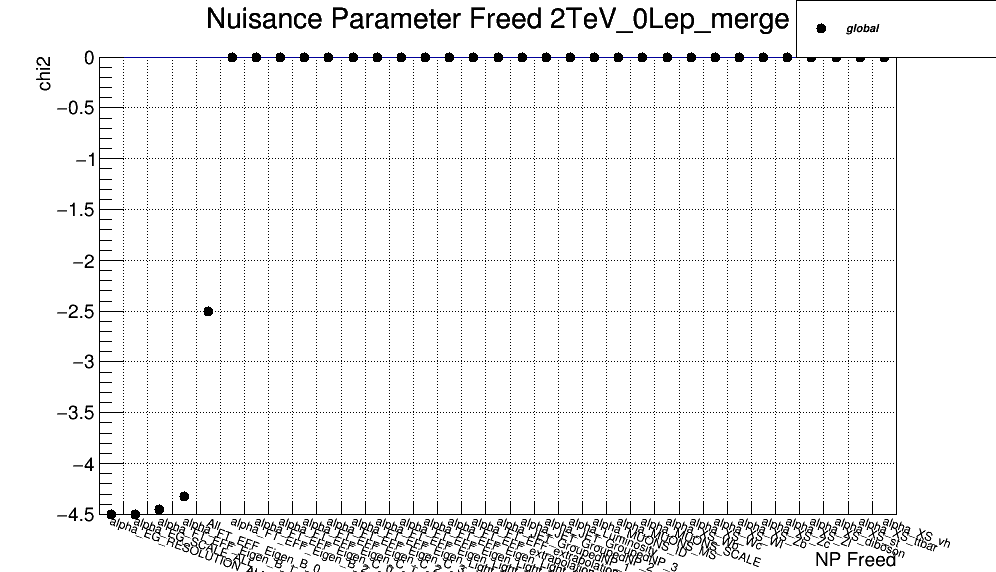
\includegraphics[width=0.8\linewidth]{pics/globalFitMu_2TeV_0Lep_merge.png}\\
\tiny{ Merge. Mu }\\
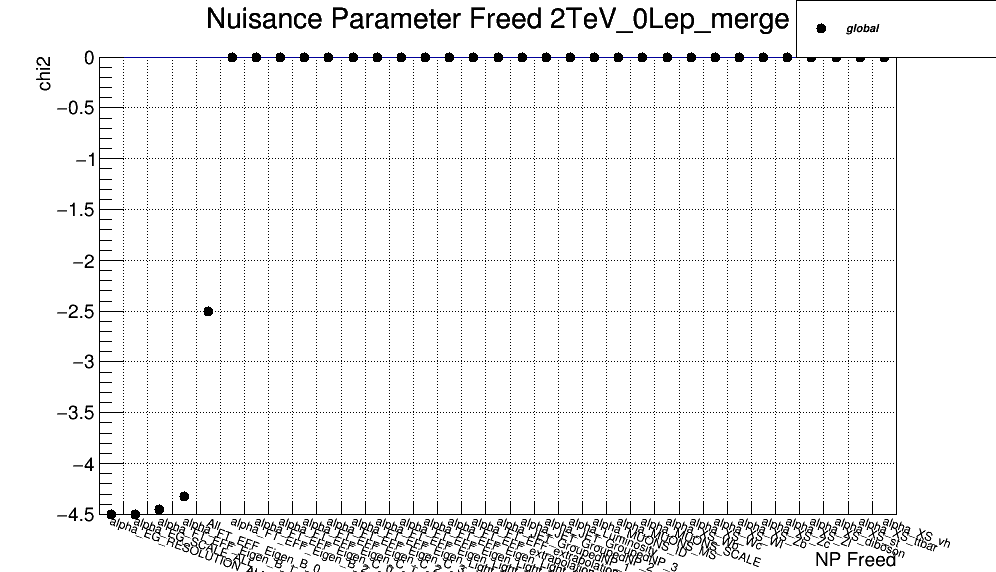
\includegraphics[width=0.8\linewidth]{pics/globalFitChi2_2TeV_0Lep_merge_.png}\\ 
\tiny{ Merge . Chi2 }\\
\end{columns}
\end{frame}

\begin{frame}
\frametitle{1 Lepton. 2TeV}
\begin{columns}[t]
\column{0.5\textwidth}
\centering
%\includegraphics[width=0.8\linewidth]{pics/globalFitMu_2TeV_1Lep_uni.png}\\
\tiny{ Uniform Mu }\\
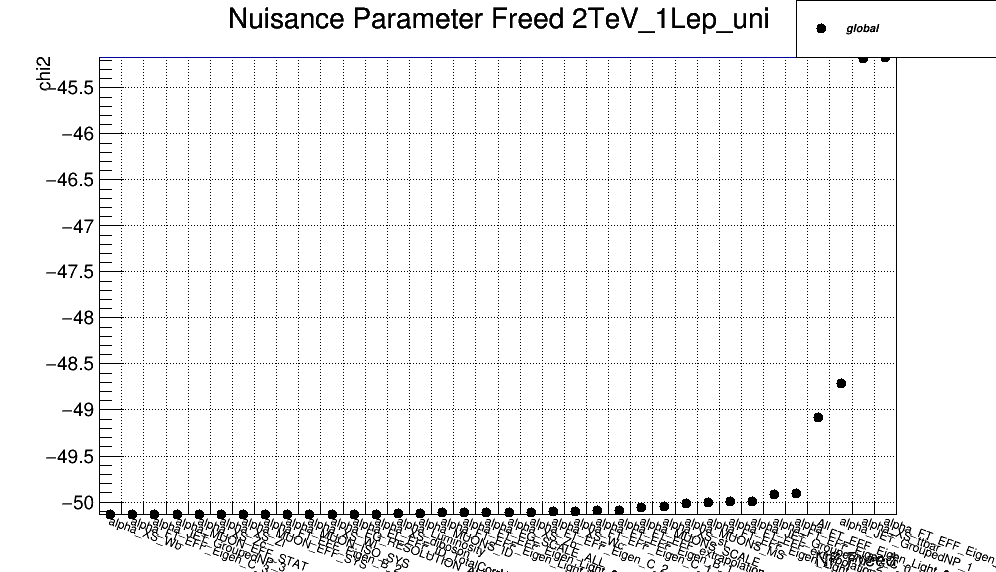
\includegraphics[width=0.8\linewidth]{pics/globalFitChi2_2TeV_1Lep_uni_.png}\\
\tiny{ Uniform. chi2  }\\
\column{0.5\textwidth}
\centering
%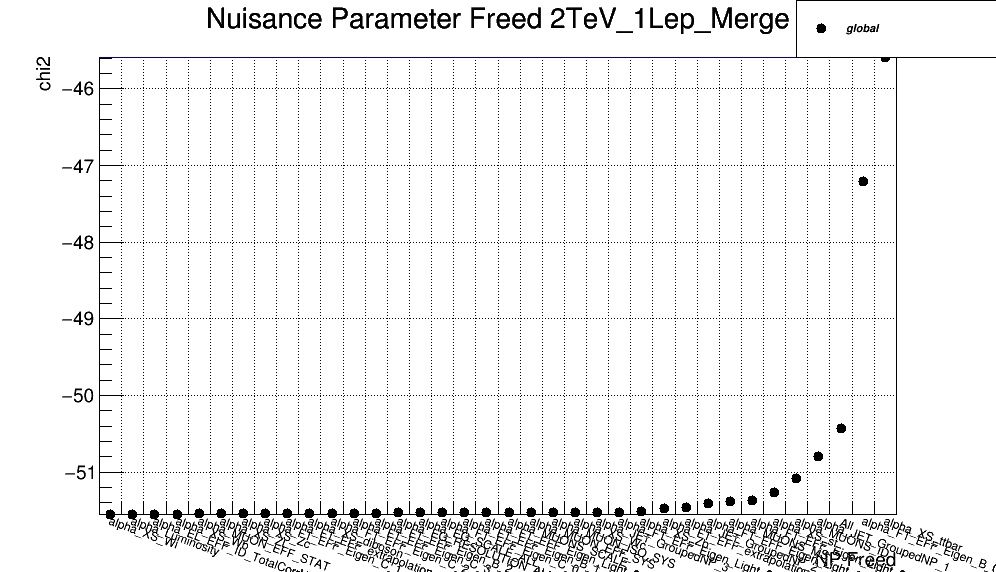
\includegraphics[width=0.8\linewidth]{pics/globalFitMu_2TeV_1Lep_Merge.png}\\
\tiny{ Merge. Mu }\\
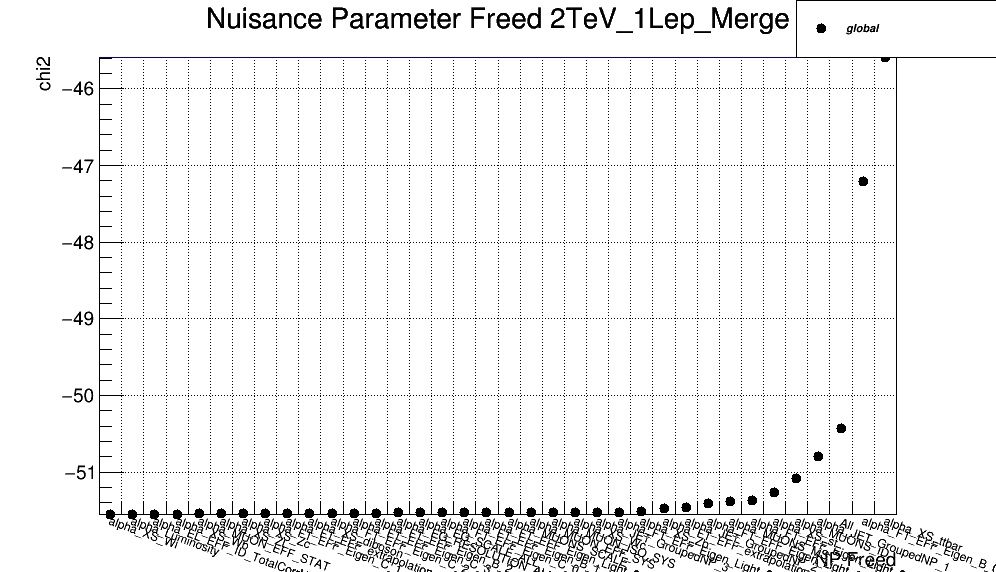
\includegraphics[width=0.8\linewidth]{pics/globalFitChi2_2TeV_1Lep_Merge_.png}\\ 
\tiny{ Merge . Chi2 }\\
\end{columns}
\end{frame}

\end{document}
\begin{frame}
\titlepage % Print the title page as the first slide
\end{frame}

\begin{frame}
\frametitle{Significance Plots}
\begin{columns}[t]
\column{0.5\textwidth}
\centering
\includegraphics[width=0.8\linewidth]{pics/Sig_1000_2000_3000_topo_mass.png}\\
\tiny{ Topo/Mass }\\
\includegraphics[width=0.8\linewidth]{pics/Sig_1000_2000_3000_topo_mass_log.png}\\
\tiny{Topo/Mass (Log) }\\
\column{0.5\textwidth}
\centering
\begin{itemize}
\item Black:1TeV
\item Green:2TeV
\item Red:3TeV
\end{itemize}
\end{columns}
\end{frame}

\begin{frame}
\frametitle{Significance Plots}
\begin{columns}[t]
\column{0.5\textwidth}
\centering
\includegraphics[width=0.8\linewidth]{pics/Sig_1000_2000_3000_Topo.png}\\
\tiny{ Topo }\\
\includegraphics[width=0.8\linewidth]{pics/Sig_1000_2000_3000_Topo_log.png}\\
\tiny{ Topo (Log)  }\\
\column{0.5\textwidth}
\centering
\includegraphics[width=0.8\linewidth]{pics/Sig_1000_2000_3000_Mass.png}\\ 
\tiny{ Mass Only }\\
\includegraphics[width=0.8\linewidth]{pics/Sig_1000_2000_3000_Mass_log.png}\\ 
\tiny{ Mass (Log) }\\
\end{columns}
\end{frame}


\begin{frame}
\frametitle{Preselection}
\begin{columns}[t]
\column{0.5\textwidth}
\centering
\includegraphics[width=0.8\linewidth]{pics/Pre/h_2TeV_2Tag_NoAdditional_pre_0_95/log_vh_m_log.pdf}\\
\tiny{ log VH Mass }\\
\includegraphics[width=0.8\linewidth]{pics/Pre/h_2TeV_2Tag_NoAdditional_pre_0_95/higgs_m.pdf}\\
\tiny{ ljet  }\\
\column{0.5\textwidth}
\centering
\includegraphics[width=0.8\linewidth]{pics/Pre/h_2TeV_2Tag_NoAdditional_pre_0_95/vh_pt_div_scal_sumpt.png}\\ 
\tiny{ Topo }\\
\includegraphics[width=0.8\linewidth]{pics/Pre/h_2TeV_2Tag_NoAdditional_pre_0_95/vh_pt_div_scal_sumpt_log.png}\\ 
\tiny{ Log Topo }\\
\end{columns}
\end{frame}

\begin{frame}
\frametitle{Mass Only  Eff=0.95}
\begin{columns}[t]
\column{0.5\textwidth}
\centering
\includegraphics[width=0.8\linewidth]{pics/2TeVMassEff80Up/h_2TeV_2Tag_NoAdditional_Mass_VHCut_0_95/log_vh_m_log.pdf}\\
\tiny{ log VH Mass }\\
\includegraphics[width=0.8\linewidth]{pics/2TeVMassEff80Up/h_2TeV_2Tag_NoAdditional_Mass_VHCut_0_95/higgs_m.pdf}\\
\tiny{ ljet  }\\
\column{0.5\textwidth}
\centering
\includegraphics[width=0.8\linewidth]{pics/2TeVMassEff80Up/h_2TeV_2Tag_NoAdditional_Mass_VHCut_0_95/vh_pt_div_scal_sumpt.png}\\ 
\tiny{ Topo }\\
\includegraphics[width=0.8\linewidth]{pics/2TeVMassEff80Up/h_2TeV_2Tag_NoAdditional_Mass_VHCut_0_95/vh_pt_div_scal_sumpt_log.png}\\ 
\tiny{ Log Topo }\\
\end{columns}
\end{frame}

\begin{frame}
\frametitle{Mass Only  Eff=0.90}
\begin{columns}[t]
\column{0.5\textwidth}
\centering
\includegraphics[width=0.8\linewidth]{pics/2TeVMassEff80Up/h_2TeV_2Tag_NoAdditional_Mass_VHCut_0_9/log_vh_m_log.pdf}\\
\tiny{ log VH Mass }\\
\includegraphics[width=0.8\linewidth]{pics/2TeVMassEff80Up/h_2TeV_2Tag_NoAdditional_Mass_VHCut_0_9/higgs_m.pdf}\\
\tiny{ ljet  }\\
\column{0.5\textwidth}
\centering
\includegraphics[width=0.8\linewidth]{pics/2TeVMassEff80Up/h_2TeV_2Tag_NoAdditional_Mass_VHCut_0_9/vh_pt_div_scal_sumpt.png}\\ 
\tiny{ Topo }\\
\includegraphics[width=0.8\linewidth]{pics/2TeVMassEff80Up/h_2TeV_2Tag_NoAdditional_Mass_VHCut_0_9/vh_pt_div_scal_sumpt_log.png}\\ 
\tiny{ Log Topo }\\
\end{columns}
\end{frame}

\begin{frame}
\frametitle{Mass Only  Eff=0.85}
\begin{columns}[t]
\column{0.5\textwidth}
\centering
\includegraphics[width=0.8\linewidth]{pics/2TeVMassEff80Up/h_2TeV_2Tag_NoAdditional_Mass_VHCut_0_85/log_vh_m_log.pdf}\\
\tiny{ log VH Mass }\\
\includegraphics[width=0.8\linewidth]{pics/2TeVMassEff80Up/h_2TeV_2Tag_NoAdditional_Mass_VHCut_0_85/higgs_m.pdf}\\
\tiny{ ljet  }\\
\column{0.5\textwidth}
\centering
\includegraphics[width=0.8\linewidth]{pics/2TeVMassEff80Up/h_2TeV_2Tag_NoAdditional_Mass_VHCut_0_85/vh_pt_div_scal_sumpt.png}\\ 
\tiny{ Topo }\\
\includegraphics[width=0.8\linewidth]{pics/2TeVMassEff80Up/h_2TeV_2Tag_NoAdditional_Mass_VHCut_0_85/vh_pt_div_scal_sumpt_log.png}\\ 
\tiny{ Log Topo }\\
\end{columns}
\end{frame}

\begin{frame}
\frametitle{Mass Only  Eff=0.80}
\begin{columns}[t]
\column{0.5\textwidth}
\centering
\includegraphics[width=0.8\linewidth]{pics/2TeVMassEff80Up/h_2TeV_2Tag_NoAdditional_Mass_VHCut_0_8/log_vh_m_log.pdf}\\
\tiny{ log VH Mass }\\
\includegraphics[width=0.8\linewidth]{pics/2TeVMassEff80Up/h_2TeV_2Tag_NoAdditional_Mass_VHCut_0_8/higgs_m.pdf}\\
\tiny{ ljet  }\\
\column{0.5\textwidth}
\centering
\includegraphics[width=0.8\linewidth]{pics/2TeVMassEff80Up/h_2TeV_2Tag_NoAdditional_Mass_VHCut_0_8/vh_pt_div_scal_sumpt.png}\\ 
\tiny{ Topo }\\
\includegraphics[width=0.8\linewidth]{pics/2TeVMassEff80Up/h_2TeV_2Tag_NoAdditional_Mass_VHCut_0_8/vh_pt_div_scal_sumpt_log.png}\\ 
\tiny{ Log Topo }\\
\end{columns}
\end{frame}

%%%%%%%%%%%%%%%%%%%%%%%%%%%%%%%%%%%%%Topo only

\begin{frame}
\frametitle{Topo Only  Eff=0.95}
\begin{columns}[t]
\column{0.5\textwidth}
\centering
\includegraphics[width=0.8\linewidth]{pics/2TeVTopoEff80Up/h_2TeV_2Tag_NoAdditional_Topo_VHCut_0_95/log_vh_m_log.pdf}\\
\tiny{ log VH Mass }\\
\includegraphics[width=0.8\linewidth]{pics/2TeVTopoEff80Up/h_2TeV_2Tag_NoAdditional_Topo_VHCut_0_95/higgs_m.pdf}\\
\tiny{ ljet  }\\
\column{0.5\textwidth}
\centering
\includegraphics[width=0.8\linewidth]{pics/2TeVTopoEff80Up/h_2TeV_2Tag_NoAdditional_Topo_VHCut_0_95/vh_pt_div_scal_sumpt.png}\\ 
\tiny{ Topo }\\
\includegraphics[width=0.8\linewidth]{pics/2TeVTopoEff80Up/h_2TeV_2Tag_NoAdditional_Topo_VHCut_0_95/vh_pt_div_scal_sumpt_log.png}\\ 
\tiny{ Log Topo }\\
\end{columns}
\end{frame}

\begin{frame}
\frametitle{Topo Only  Eff=0.90}
\begin{columns}[t]
\column{0.5\textwidth}
\centering
\includegraphics[width=0.8\linewidth]{pics/2TeVTopoEff80Up/h_2TeV_2Tag_NoAdditional_Topo_VHCut_0_9/log_vh_m_log.pdf}\\
\tiny{ log VH Mass }\\
\includegraphics[width=0.8\linewidth]{pics/2TeVTopoEff80Up/h_2TeV_2Tag_NoAdditional_Topo_VHCut_0_9/higgs_m.pdf}\\
\tiny{ ljet  }\\
\column{0.5\textwidth}
\centering
\includegraphics[width=0.8\linewidth]{pics/2TeVTopoEff80Up/h_2TeV_2Tag_NoAdditional_Topo_VHCut_0_9/vh_pt_div_scal_sumpt.png}\\ 
\tiny{ Topo }\\
\includegraphics[width=0.8\linewidth]{pics/2TeVTopoEff80Up/h_2TeV_2Tag_NoAdditional_Topo_VHCut_0_9/vh_pt_div_scal_sumpt_log.png}\\ 
\tiny{ Log Topo }\\
\end{columns}
\end{frame}

\begin{frame}
\frametitle{Topo Only  Eff=0.85}
\begin{columns}[t]
\column{0.5\textwidth}
\centering
\includegraphics[width=0.8\linewidth]{pics/2TeVTopoEff80Up/h_2TeV_2Tag_NoAdditional_Topo_VHCut_0_85/log_vh_m_log.pdf}\\
\tiny{ log VH Mass }\\
\includegraphics[width=0.8\linewidth]{pics/2TeVTopoEff80Up/h_2TeV_2Tag_NoAdditional_Topo_VHCut_0_85/higgs_m.pdf}\\
\tiny{ ljet  }\\
\column{0.5\textwidth}
\centering
\includegraphics[width=0.8\linewidth]{pics/2TeVTopoEff80Up/h_2TeV_2Tag_NoAdditional_Topo_VHCut_0_85/vh_pt_div_scal_sumpt.png}\\ 
\tiny{ Topo }\\
\includegraphics[width=0.8\linewidth]{pics/2TeVTopoEff80Up/h_2TeV_2Tag_NoAdditional_Topo_VHCut_0_85/vh_pt_div_scal_sumpt_log.png}\\ 
\tiny{ Log Topo }\\
\end{columns}
\end{frame}

\begin{frame}
\frametitle{Topo Only  Eff=0.80}
\begin{columns}[t]
\column{0.5\textwidth}
\centering
\includegraphics[width=0.8\linewidth]{pics/2TeVTopoEff80Up/h_2TeV_2Tag_NoAdditional_Topo_VHCut_0_8/log_vh_m_log.pdf}\\
\tiny{ log VH Mass }\\
\includegraphics[width=0.8\linewidth]{pics/2TeVTopoEff80Up/h_2TeV_2Tag_NoAdditional_Topo_VHCut_0_8/higgs_m.pdf}\\
\tiny{ ljet  }\\
\column{0.5\textwidth}
\centering
\includegraphics[width=0.8\linewidth]{pics/2TeVTopoEff80Up/h_2TeV_2Tag_NoAdditional_Topo_VHCut_0_8/vh_pt_div_scal_sumpt.png}\\ 
\tiny{ Topo }\\
\includegraphics[width=0.8\linewidth]{pics/2TeVTopoEff80Up/h_2TeV_2Tag_NoAdditional_Topo_VHCut_0_8/vh_pt_div_scal_sumpt_log.png}\\ 
\tiny{ Log Topo }\\
\end{columns}
\end{frame}

%%%%%%%%%%%%%%%%%%%%%%%%%%%%%%%%%%%%%%%%%%%%%%  Topo + Mass

\begin{frame}
\frametitle{Topo/Mass  Eff=0.95}
\begin{columns}[t]
\column{0.5\textwidth}
\centering
\includegraphics[width=0.8\linewidth]{pics/2TeVMassTopoEff80Up/h_2TeV_2Tag_NoAdditional_Topo_Mass_VHCut_0_95/log_vh_m_log.pdf}\\
\tiny{ log VH Mass }\\
\includegraphics[width=0.8\linewidth]{pics/2TeVMassTopoEff80Up/h_2TeV_2Tag_NoAdditional_Topo_Mass_VHCut_0_95/higgs_m.pdf}\\
\tiny{ ljet  }\\
\column{0.5\textwidth}
\centering
\includegraphics[width=0.8\linewidth]{pics/2TeVMassTopoEff80Up/h_2TeV_2Tag_NoAdditional_Topo_Mass_VHCut_0_95/vh_pt_div_scal_sumpt.png}\\ 
\tiny{ Topo }\\
\includegraphics[width=0.8\linewidth]{pics/2TeVMassTopoEff80Up/h_2TeV_2Tag_NoAdditional_Topo_Mass_VHCut_0_95/vh_pt_div_scal_sumpt_log.png}\\ 
\tiny{ Log Topo }\\
\end{columns}
\end{frame}

\begin{frame}
\frametitle{Topo/Mass  Eff=0.90}
\begin{columns}[t]
\column{0.5\textwidth}
\centering
\includegraphics[width=0.8\linewidth]{pics/2TeVMassTopoEff80Up/h_2TeV_2Tag_NoAdditional_Topo_Mass_VHCut_0_9/log_vh_m_log.pdf}\\
\tiny{ log VH Mass }\\
\includegraphics[width=0.8\linewidth]{pics/2TeVMassTopoEff80Up/h_2TeV_2Tag_NoAdditional_Topo_Mass_VHCut_0_9/higgs_m.pdf}\\
\tiny{ ljet  }\\
\column{0.5\textwidth}
\centering
\includegraphics[width=0.8\linewidth]{pics/2TeVMassTopoEff80Up/h_2TeV_2Tag_NoAdditional_Topo_Mass_VHCut_0_9/vh_pt_div_scal_sumpt.png}\\ 
\tiny{ Topo }\\
\includegraphics[width=0.8\linewidth]{pics/2TeVMassTopoEff80Up/h_2TeV_2Tag_NoAdditional_Topo_Mass_VHCut_0_9/vh_pt_div_scal_sumpt_log.png}\\ 
\tiny{ Log Topo }\\
\end{columns}
\end{frame}

\begin{frame}
\frametitle{Topo/Mass  Eff=0.85}
\begin{columns}[t]
\column{0.5\textwidth}
\centering
\includegraphics[width=0.8\linewidth]{pics/2TeVMassTopoEff80Up/h_2TeV_2Tag_NoAdditional_Topo_Mass_VHCut_0_85/log_vh_m_log.pdf}\\
\tiny{ log VH Mass }\\
\includegraphics[width=0.8\linewidth]{pics/2TeVMassTopoEff80Up/h_2TeV_2Tag_NoAdditional_Topo_Mass_VHCut_0_85/higgs_m.pdf}\\
\tiny{ ljet  }\\
\column{0.5\textwidth}
\centering
\includegraphics[width=0.8\linewidth]{pics/2TeVMassTopoEff80Up/h_2TeV_2Tag_NoAdditional_Topo_Mass_VHCut_0_85/vh_pt_div_scal_sumpt.png}\\ 
\tiny{ Topo }\\
\includegraphics[width=0.8\linewidth]{pics/2TeVMassTopoEff80Up/h_2TeV_2Tag_NoAdditional_Topo_Mass_VHCut_0_85/vh_pt_div_scal_sumpt_log.png}\\ 
\tiny{ Log Topo }\\
\end{columns}
\end{frame}

\begin{frame}
\frametitle{Topo/Mass  Eff=0.80}
\begin{columns}[t]
\column{0.5\textwidth}
\centering
\includegraphics[width=0.8\linewidth]{pics/2TeVMassTopoEff80Up/h_2TeV_2Tag_NoAdditional_Topo_Mass_VHCut_0_8/log_vh_m_log.pdf}\\
\tiny{ log VH Mass }\\
\includegraphics[width=0.8\linewidth]{pics/2TeVMassTopoEff80Up/h_2TeV_2Tag_NoAdditional_Topo_Mass_VHCut_0_8/higgs_m.pdf}\\
\tiny{ ljet  }\\
\column{0.5\textwidth}
\centering
\includegraphics[width=0.8\linewidth]{pics/2TeVMassTopoEff80Up/h_2TeV_2Tag_NoAdditional_Topo_Mass_VHCut_0_8/vh_pt_div_scal_sumpt.png}\\ 
\tiny{ Topo }\\
\includegraphics[width=0.8\linewidth]{pics/2TeVMassTopoEff80Up/h_2TeV_2Tag_NoAdditional_Topo_Mass_VHCut_0_8/vh_pt_div_scal_sumpt_log.png}\\ 
\tiny{ Log Topo }\\
\end{columns}
\end{frame}





%%%%%%%%%%%%%%%%%%%%%%%%%%%%%%%%%%%%%%%%%%%%%%%%%%%%%

\begin{frame}
backup
\end{frame}


\begin{frame}
\frametitle{Mass Only  Eff=0.8/0.6 }
\begin{columns}[t]
\column{0.5\textwidth}
\centering
\includegraphics[width=0.8\linewidth]{pics/2TeVMass/h_2TeV_2Tag_NoAdditional_Mass_VHCut_0_8/log_vh_m_log.pdf}\\
\tiny{ log VH Mass Eff=0.8 }\\
\includegraphics[width=0.8\linewidth]{pics/2TeVMass/h_2TeV_2Tag_NoAdditional_Mass_VHCut_0_8/higgs_m.pdf}\\
\tiny{ ljet Eff=0.8 }\\
\column{0.5\textwidth}
\centering
\includegraphics[width=0.8\linewidth]{pics/2TeVMass/h_2TeV_2Tag_NoAdditional_Mass_VHCut_0_6/log_vh_m_log.pdf}\\ 
\tiny{ log VH Mass Eff=0.6 }\\
\centering
\includegraphics[width=0.8\linewidth]{pics/2TeVMass/h_2TeV_2Tag_NoAdditional_Mass_VHCut_0_6/higgs_m.pdf}\\ 
\tiny{ ljet Eff=0.6 }\\
\end{columns}
\end{frame}

\begin{frame}
\frametitle{Mass Only  Eff=0.4/0.2 }
\begin{columns}[t]
\column{0.5\textwidth}
\centering
\includegraphics[width=0.8\linewidth]{pics/2TeVMass/h_2TeV_2Tag_NoAdditional_Mass_VHCut_0_4/log_vh_m_log.pdf}\\
\tiny{ log VH Mass Eff=0.6 }\\
\includegraphics[width=0.8\linewidth]{pics/2TeVMass/h_2TeV_2Tag_NoAdditional_Mass_VHCut_0_4/higgs_m.pdf}\\
\tiny{ ljet Eff=0.6 }\\
\column{0.5\textwidth}
\centering
\includegraphics[width=0.8\linewidth]{pics/2TeVMass/h_2TeV_2Tag_NoAdditional_Mass_VHCut_0_2/log_vh_m_log.pdf}\\ 
\tiny{ log VH Mass Eff=0.4 }\\
\centering
\includegraphics[width=0.8\linewidth]{pics/2TeVMass/h_2TeV_2Tag_NoAdditional_Mass_VHCut_0_2/higgs_m.pdf}\\ 
\tiny{ ljet Eff=0.4 }\\
\end{columns}
\end{frame}

\begin{frame}
\frametitle{Topo  Eff=0.8/0.6 }
\begin{columns}[t]
\column{0.5\textwidth}
\centering
\includegraphics[width=0.8\linewidth]{pics/2TeVTopo/h_2TeV_2Tag_NoAdditional_Topo_VHCut_0_8/log_vh_m_log.pdf}\\
\tiny{ log VH Mass Eff=0.8 }\\
\includegraphics[width=0.8\linewidth]{pics/2TeVTopo/h_2TeV_2Tag_NoAdditional_Topo_VHCut_0_8/higgs_m.pdf}\\
\tiny{ ljet Eff=0.8 }\\
\column{0.5\textwidth}
\centering
\includegraphics[width=0.8\linewidth]{pics/2TeVTopo/h_2TeV_2Tag_NoAdditional_Topo_VHCut_0_6/log_vh_m_log.pdf}\\ 
\tiny{ log VH Mass Eff=0.6 }\\
\centering
\includegraphics[width=0.8\linewidth]{pics/2TeVTopo/h_2TeV_2Tag_NoAdditional_Topo_VHCut_0_6/higgs_m.pdf}\\ 
\tiny{ ljet Eff=0.6 }\\
\end{columns}
\end{frame}

\begin{frame}
\frametitle{Topo  Eff=0.4/0.2 }
\begin{columns}[t]
\column{0.5\textwidth}
\centering
\includegraphics[width=0.8\linewidth]{pics/2TeVTopo/h_2TeV_2Tag_NoAdditional_Topo_VHCut_0_4/log_vh_m_log.pdf}\\
\tiny{ log VH Mass Eff=0.4 }\\
\includegraphics[width=0.8\linewidth]{pics/2TeVTopo/h_2TeV_2Tag_NoAdditional_Topo_VHCut_0_4/higgs_m.pdf}\\
\tiny{ ljet Eff=0.4 }\\
\column{0.5\textwidth}
\centering
\includegraphics[width=0.8\linewidth]{pics/2TeVTopo/h_2TeV_2Tag_NoAdditional_Topo_VHCut_0_2/log_vh_m_log.pdf}\\ 
\tiny{ log VH Mass Eff=0.2 }\\
\centering
\includegraphics[width=0.8\linewidth]{pics/2TeVTopo/h_2TeV_2Tag_NoAdditional_Topo_VHCut_0_2/higgs_m.pdf}\\ 
\tiny{ ljet Eff=0.2 }\\
\end{columns}
\end{frame}


\begin{frame}
\frametitle{Topo/Mass  Eff=0.8/0.6 }
\begin{columns}[t]
\column{0.5\textwidth}
\centering
\includegraphics[width=0.8\linewidth]{pics/2TeVMassTopo/h_2TeV_2Tag_NoAdditional_Topo_Mass_VHCut_0_8/log_vh_m_log.pdf}\\
\tiny{ log VH Mass Eff=0.8 }\\
\includegraphics[width=0.8\linewidth]{pics/2TeVMassTopo/h_2TeV_2Tag_NoAdditional_Topo_Mass_VHCut_0_8/higgs_m.pdf}\\
\tiny{ ljet Eff=0.8 }\\
\column{0.5\textwidth}
\centering
\includegraphics[width=0.8\linewidth]{pics/2TeVMassTopo/h_2TeV_2Tag_NoAdditional_Topo_Mass_VHCut_0_6/log_vh_m_log.pdf}\\ 
\tiny{ log VH Mass Eff=0.6 }\\
\centering
\includegraphics[width=0.8\linewidth]{pics/2TeVMassTopo/h_2TeV_2Tag_NoAdditional_Topo_Mass_VHCut_0_6/higgs_m.pdf}\\ 
\tiny{ ljet Eff=0.6 }\\
\end{columns}
\end{frame}

\begin{frame}
\frametitle{Topo/Mass  Eff=0.4/0.2 }
\begin{columns}[t]
\column{0.5\textwidth}
\centering
\includegraphics[width=0.8\linewidth]{pics/2TeVMassTopo/h_2TeV_2Tag_NoAdditional_Topo_Mass_VHCut_0_4/log_vh_m_log.pdf}\\
\tiny{ log VH Mass Eff=0.4 }\\
\includegraphics[width=0.8\linewidth]{pics/2TeVMassTopo/h_2TeV_2Tag_NoAdditional_Topo_Mass_VHCut_0_4/higgs_m.pdf}\\
\tiny{ ljet Eff=0.4 }\\
\column{0.5\textwidth}
\centering
\includegraphics[width=0.8\linewidth]{pics/2TeVMassTopo/h_2TeV_2Tag_NoAdditional_Topo_Mass_VHCut_0_2/log_vh_m_log.pdf}\\ 
\tiny{ log VH Mass Eff=0.2 }\\
\centering
\includegraphics[width=0.8\linewidth]{pics/2TeVMassTopo/h_2TeV_2Tag_NoAdditional_Topo_Mass_VHCut_0_2/higgs_m.pdf}\\ 
\tiny{ ljet Eff=0.2 }\\
\end{columns}
\end{frame}


\begin{frame}
\frametitle{Introduction} 
\begin{tcolorbox}[title = Plan]
Window cuts based classification used to investigate optimisation of topology/mass variable.
Interested in how much the topology cut adds to the expected significance. TMVA was used for this purpose.
\end{tcolorbox}
\begin{columns}
\column{0.5\textwidth}
\begin{tcolorbox}[ colback=red!5!white,colframe=red!75!black,title=Samples]
\begin{itemize}
\item HVT $\rightarrow$ WH $\rightarrow$ e/$\mu$ $\nu$ qq
\item 1/2/3 TeV resonance mass
\end{itemize}
\end{tcolorbox}
\column{0.5\textwidth}
\begin{tcolorbox}[ colback=red!5!white,colframe=red!75!black,title=Variables]
 \begin{enumerate}
	\item  topo = $\frac{VH_{pt}}{V_{pt} + H_{pt}}$
	\item $m_{H}$ (Fat Jet)
\end{enumerate}
\end{tcolorbox}
\end{columns}
\end{frame}

\begin{frame}
\frametitle{Preselection}
Performed before optimisation:
 \begin{enumerate}
	\item  25 GeV electron or muon 
	\item  2 B-tagged track jets in fat jet
	\item No additional b-tagged tracks jets outside fat jet. 
	\item Higgs mass window cut: ( 75 GeV $<$ ljet $<$ 145 GeV )
	\item VH mass cut over 1 TeV. 
\end{enumerate}
\end{frame}

\begin{frame}
\frametitle{ROC 1/2/3 TeV.}
\begin{columns}[t]
\column{0.5\textwidth}
\centering
\includegraphics[width=0.8\linewidth]{pics/output/config-ROCMC15.png}\\
\tiny{1 TeV }\\
\includegraphics[width=0.8\linewidth]{pics/output/config-2TeV.png}\\
\tiny{2 TeV }
\column{0.5\textwidth}
\centering
\includegraphics[width=0.8\linewidth]{pics/output/config-3TeV.png}\\
\tiny{3 TeV }\\ 
Trained for each variable and then the combination.
\newline
\newline
\textcolor{black}{Black}$=>$Combination
\newline
\textcolor{red}{Red}$=>$Topo Only 
\newline
\textcolor{green}{Green}$=>$Mass Only
\newline
\end{columns} 
\end{frame}

\begin{frame}
\frametitle{Mass Trained Only.}
\begin{columns}[t]
\column{0.5\textwidth}
\centering
\includegraphics[width=0.8\linewidth]{pics/output/1TeV_2Tag_NoAdditional_Mass_Add/Cuts0.png}\\
\tiny{1 TeV }\\
\includegraphics[width=0.8\linewidth]{pics/output/2TeV_2Tag_NoAdditional_Mass_Add/Cuts0.png}\\
\tiny{2 TeV }\\
\column{0.5\textwidth}
\centering
\includegraphics[width=0.8\linewidth]{pics/output/3TeV_2Tag_NoAdditional_Mass_Add/Cuts0.png}\\
\tiny{3 TeV }\\
\hfill \break
\textcolor{black}{Black}/\textcolor{red}{Red} denote Min/Max cut. 
\newline
Interested in behaviour of cuts with signal acceptance.
\newline
 This is related to the green ROC previously shown.
\end{columns}

\end{frame}

\begin{frame}
\frametitle{Topo Trained Only.}
\begin{columns}[t]
\column{0.5\textwidth}
\centering
\includegraphics[width=0.8\linewidth]{pics/output/1TeV_2Tag_NoAdditional_Topo_Add/Cuts0.png}\\
\tiny{1 TeV }\\
\includegraphics[width=0.8\linewidth]{pics/output/2TeV_2Tag_NoAdditional_Topo_Add/Cuts0.png}\\
\tiny{2 TeV }\\
\column{0.5\textwidth}
\centering
\includegraphics[width=0.8\linewidth]{pics/output/3TeV_2Tag_NoAdditional_Topo_Add/Cuts0.png}\\
\tiny{3 TeV }\\
\hfill \break
Same again but this time for the topo variable trained only now.
\end{columns}

\end{frame}

\begin{frame}
\frametitle{Topo/Mass Trained 1/2 TeV}
\begin{columns}[t]
\column{0.5\textwidth}
\centering
\includegraphics[width=0.8\linewidth]{pics/output/1TeV_2Tag_NoAdditional_Topo_Mass_Add/Cuts0.png}\\
\tiny{1 TeV (Topo) }\\
\includegraphics[width=0.8\linewidth]{pics/output/1TeV_2Tag_NoAdditional_Topo_Mass_Add/Cuts1.png}\\
\tiny{1 TeV (Mass) }\\
\column{0.5\textwidth}
\centering
\includegraphics[width=0.8\linewidth]{pics/output/2TeV_2Tag_NoAdditional_Topo_Mass__Add/Cuts0.png}\\
\tiny{2 TeV (Topo) }\\
\includegraphics[width=0.8\linewidth]{pics/output/2TeV_2Tag_NoAdditional_Topo_Mass__Add/Cuts1.png}\\
\tiny{2 TeV (Mass) }\\
\end{columns}
\end{frame}

\begin{frame}
\frametitle{Topo/Mass Trained 3 TeV}
\centering
\includegraphics[width=0.5\linewidth]{pics/output/3TeV_2Tag_NoAdditional_Topo_Mass_Add/Cuts0.png}
\includegraphics[width=0.5\linewidth]{pics/output/3TeV_2Tag_NoAdditional_Topo_Mass_Add/Cuts1.png}
\newline
3 TeV (Left Topo, Right Mass)
\end{frame}

\begin{frame}
\frametitle{Significance for 2TeV}
\begin{columns}[t]
\column{0.5\textwidth}
\centering
\includegraphics[width=0.8\linewidth]{pics/output/2_TeV_HVT_res-Mass.png}\\
\tiny{Mass Only }\\
\includegraphics[width=0.8\linewidth]{pics/output/2_TeV_HVT_res-Topo.png}\\
\tiny{Topo Only }\\
\column{0.5\textwidth}
\centering
\includegraphics[width=0.8\linewidth]{pics/output/2_TeV_HVT_res-Topo-Mass.png}\\
\tiny{Topo and Mass }\\


\hfill \break
\begin{itemize}
\item Significance defined as quadrature sum of $\frac{S}{\sqrt{B}}$. 
\item Significance is calculated for each set of cuts at each efficiency.
\item Each colour a different mass point using the cuts for the 2TeV training.
\item The post cuts plot I do not have yet to estimate expected significance
\end{itemize}
\end{columns}
\end{frame}

\begin{frame}
\frametitle{Significance for 1TeV }
\begin{columns}[t]
\column{0.5\textwidth}
\centering
\includegraphics[width=0.8\linewidth]{pics/output/1_TeV_HVT_res-Mass.png}\\
\tiny{Mass Only }\\
\includegraphics[width=0.8\linewidth]{pics/output/1_TeV_HVT_res-Topo.png}\\
\tiny{Topo Only }\\
\column{0.5\textwidth}
\centering
\includegraphics[width=0.8\linewidth]{pics/output/1_TeV_HVT_res-Topo-Mass.png}\\ 
\tiny{Topo-Mass}\\
\end{columns}

\end{frame}

\begin{frame}
\frametitle{Distributions after Preselection Cuts }
\begin{columns}[t]
\column{0.5\textwidth}
\centering
\includegraphics[width=0.8\linewidth]{pics/vh_m_log.pdf}\\
\includegraphics[width=0.8\linewidth]{pics/vh_pt_div_scal_sumpt_log.pdf}
\column{0.5\textwidth}
\centering
\includegraphics[width=0.8\linewidth]{pics/ljet0_m_log.pdf}\\ 
All cross sections normalized to 1pb. 
\end{columns}

\end{frame}

\begin{frame}
\frametitle{1TeV Mass eff=0.9 }
\begin{columns}[t]
\column{0.5\textwidth}
\centering
\includegraphics[width=0.8\linewidth]{pics/1TeVMass/h_1TeV_2Tag_NoAdditional_Mass_Add_0_9/log_vh_m_log.png}\\
\tiny{ log(vh mass) (log) }\\
\includegraphics[width=0.8\linewidth]{pics/1TeVMass/h_1TeV_2Tag_NoAdditional_Mass_Add_0_9/vh_m.png}\\
\tiny{vh mass }\\
\column{0.5\textwidth}
\centering
\includegraphics[width=0.8\linewidth]{pics/1TeVMass/h_1TeV_2Tag_NoAdditional_Mass_Add_0_9/higgs_m.png}\\ 
\tiny{H mass}\\
\begin{itemize}
\item Cuts on 1 TeV mass
\end{itemize}
\end{columns}
\end{frame}

\begin{frame}
\frametitle{1TeV Mass eff=0.9 }
\begin{columns}[t]
\column{0.5\textwidth}
\centering
\includegraphics[width=0.8\linewidth]{pics/1TeVMass/h_1TeV_2Tag_NoAdditional_Mass_Add_0_9/log_vh_m_log.png}\\
\tiny{ log(vh mass) (log) }\\
\includegraphics[width=0.8\linewidth]{pics/1TeVMass/h_1TeV_2Tag_NoAdditional_Mass_Add_0_9/vh_m.png}\\
\tiny{vh mass }\\
\column{0.5\textwidth}
\centering
\includegraphics[width=0.8\linewidth]{pics/1TeVMass/h_1TeV_2Tag_NoAdditional_Mass_Add_0_9/higgs_m.png}\\ 
\tiny{H mass}\\
\begin{itemize}
\item Cuts on 1 TeV mass
\end{itemize}
\end{columns}
\end{frame}

\begin{frame}
\frametitle{Conclusion}
\begin{itemize}
\item Produce post cut plots
\item Ensure significance plots are correct
\item Investigate low stats
\end{itemize}


\end{frame}

\begin{frame}
Backup
\end{frame}

\begin{frame}
\frametitle{1TeV mass point trained.}
\begin{columns}[t]
\column{0.5\textwidth}
\centering
\includegraphics[width=0.8\linewidth]{pics/output/1TeV_2Tag_NoAdditional_Mass_Add/Cuts0.png}\\
\includegraphics[width=0.8\linewidth]{pics/output/1TeV_2Tag_NoAdditional_Topo_Add/Cuts0.png}
\column{0.5\textwidth}
\centering
\includegraphics[width=0.8\linewidth]{pics/output/1TeV_2Tag_NoAdditional_Topo_Mass_Add/Cuts0.png}\\
\includegraphics[width=0.8\linewidth]{pics/output/1TeV_2Tag_NoAdditional_Topo_Mass_Add/Cuts1.png}
\end{columns}
\small{Efficiencies are measured after box cuts on the variables of interest. This is done together and separately. (Top left going clockwise: Mass cut only, Topo + Mass(Topo variable), Topo + Mass(Mass variable), Topo cut only) }

\end{frame}

\begin{frame}
\frametitle{2TeV mass point trained.}
\begin{columns}[t]
\column{0.5\textwidth}
\centering
\includegraphics[width=0.8\linewidth]{pics/output/2TeV_2Tag_NoAdditional_Mass_Add/Cuts0.png}\\
\includegraphics[width=0.8\linewidth]{pics/output/2TeV_2Tag_NoAdditional_Topo_Add/Cuts0.png}
\column{0.5\textwidth}
\centering
\includegraphics[width=0.8\linewidth]{pics/output/2TeV_2Tag_NoAdditional_Topo_Mass__Add/Cuts0.png}\\
\includegraphics[width=0.8\linewidth]{pics/output/2TeV_2Tag_NoAdditional_Topo_Mass__Add/Cuts1.png}
\end{columns}
(Top left going clockwise: Mass cut only, Topo + Mass(Topo variable), Topo + Mass(Mass variable), Topo cut only)

\end{frame}


\begin{frame}
\frametitle{3TeV mass point trained.}
\begin{columns}[t]
\column{0.5\textwidth}
\centering
\includegraphics[width=0.8\linewidth]{pics/output/3TeV_2Tag_NoAdditional_Mass_Add/Cuts0.png}\\
\includegraphics[width=0.8\linewidth]{pics/output/3TeV_2Tag_NoAdditional_Topo_Add/Cuts0.png}
\column{0.5\textwidth}
\centering
\includegraphics[width=0.8\linewidth]{pics/output/3TeV_2Tag_NoAdditional_Topo_Mass_Add/Cuts0.png}\\
\includegraphics[width=0.8\linewidth]{pics/output/3TeV_2Tag_NoAdditional_Topo_Mass_Add/Cuts1.png}
\end{columns}
(Top left going clockwise: Mass cut only, Topo + Mass(Topo variable), Topo + Mass(Mass variable), Topo cut only)
\end{frame}





\end{document} 